\documentclass[11pt,a4paper]{article}
\usepackage[utf8]{vietnam}
\usepackage{amsmath,amssymb,mathrsfs}
\usepackage{graphicx}
\usepackage{tikz}
\usepackage{array}
\usepackage[top=1.0cm,bottom=1.8cm,left=1.4cm,right=1.4cm,footskip=0.8cm]{geometry}
\usepackage{fancyhdr}
\usepackage{tcolorbox}
\tcbuselibrary{skins}
\usepackage[dethi]{ex_test}

\makeatletter
\@ifundefined{c@bt}{\newcounter{bt}}{}
\makeatother

\pagestyle{fancy}
\fancyhf{}
\renewcommand{\headrulewidth}{0pt}
\renewcommand{\footrulewidth}{0.4pt}
\lfoot{\footnotesize\textsl{Lớp Toán Cô Thúy -- SĐT: 0935.322.328 -- 50/2C Phạm Thị Liên}}
\rfoot{\footnotesize\textsl{Trang \thepage/4 -- Mã đề 101}}

\setlength{\parskip}{0pt}

\begin{document}

% KHUNG TIÊU ĐỀ ĐỀ KIỂM TRA
\noindent
\begin{tabular}{|p{6.6cm}|p{6.6cm}|>{\centering\arraybackslash}p{3.2cm}|}
\hline
\begin{minipage}{6.6cm}
\vspace{3pt}
\centering
{\large\bfseries\color{blue!80!black} LỚP TOÁN CÔ THÚY}\\[3pt]
\textbf{SĐT:} 0935.322.328\\[2pt]
\textbf{Địa chỉ:} 50/2C Phạm Thị Liên
\vspace{3pt}
\end{minipage}
&
\multicolumn{2}{p{10.2cm}|}{
\begin{minipage}{10.2cm}
\vspace{3pt}
\centering
{\bfseries\color{red!80!black} KIỂM TRA GIỮA KỲ I -- NĂM HỌC 2024 -- 2025}\\[3pt]
\textbf{Môn: VẬT LÍ, Lớp 10 -- THPT NGUYỄN HUỆ}\\[2pt]
\textit{Thời gian làm bài: 45 phút (Không kể thời gian phát đề)}
\vspace{3pt}
\end{minipage}
} \\
\hline
\rule{0pt}{13pt}Họ và tên thí sinh: \dotfill\rule[-3pt]{0pt}{3pt} &
\rule{0pt}{13pt}Số báo danh: \dotfill\rule[-3pt]{0pt}{3pt} &
\rule{0pt}{13pt}\textbf{Mã đề thi 101}\rule[-3pt]{0pt}{3pt} \\
\hline
\end{tabular}
\vspace{0.15cm}

\begin{flushleft}
	{\color{blue!50!green}\fbox{\fontfamily{qag}\bfseries\selectfont PHẦN I. Câu trắc nghiệm nhiều phương án lựa chọn}}
	\textit{\small (Thí sinh trả lời từ câu 1 đến câu 18. Mỗi câu hỏi thí sinh chỉ chọn một phương án.)}
\end{flushleft}
\setcounter{ex}{0}
\setcounter{bt}{0}

% Câu 1
\begin{ex}
	Đối tượng nghiên cứu của Vật lí là
	\choice
	{sự thay đổi của các chất khi kết hợp với nhau}
	{qui luật tương tác của các dạng năng lượng}
	{nghiên cứu về nhiệt động lực học}
	{\True các dạng vận động của vật chất và năng lượng}
	\loigiai{}
\end{ex}

% Câu 2
\begin{ex}
	Một vật rơi tự do từ độ cao $80\text{ m}$ xuống đất. Lấy $g = 10\text{ m/s}^2$, tốc độ vật lúc vừa chạm đất là
	\choice
	{\True $40\text{ m/s}$}
	{$20\text{ m/s}$}
	{$10\text{ m/s}$}
	{$30\text{ m/s}$}
	\loigiai{}
\end{ex}

% Câu 3
\begin{ex}
	Sự rơi tự do là
	\choice
	{\True chuyển động chỉ dưới tác dụng của trọng lực}
	{một dạng chuyển động thẳng đều}
	{chuyển động khi bỏ qua mọi lực}
	{chuyển động không chịu bất cứ lực tác dụng nào}
	\loigiai{}
\end{ex}

% Câu 4
\begin{ex}
	Trong chuyển động thẳng biến đổi đều thì
	\choice
	{vận tốc là đại lượng biến thiên theo thời gian theo quy luật hàm bậc hai}
	{\True gia tốc là đại lượng không đổi}
	{vận tốc là đại lượng không đổi}
	{gia tốc là đại lượng biến thiên theo thời gian}
	\loigiai{}
\end{ex}

% Câu 5
\begin{ex}
	Gia tốc là một đại lượng
	\choice
	{vô hướng, đặc trưng cho sự biến đổi nhanh hay chậm của chuyển động}
	{vectơ, đặc trưng cho sự biến đổi nhanh hay chậm của chuyển động}
	{vô hướng, đặc trưng cho tính không đổi của vận tốc}
	{\True vectơ, đặc trưng cho sự biến đổi nhanh hay chậm của vận tốc}
	\loigiai{}
\end{ex}

% Câu 6
\begin{ex}
	Canô chuyển động thẳng xuôi dòng từ P đến Q mất 2 giờ và ngược dòng từ Q về P mất 3 giờ. Khi nước yên lặng canô chuyển động có tốc độ $50\text{ km/h}$. Tốc độ của nước so với bờ là
	\choice
	{$12{,}5\text{ km/h}$}
	{$9\text{ km/h}$}
	{\True $10\text{ km/h}$}
	{$20\text{ km/h}$}
	\loigiai{}
\end{ex}

% Câu 7
\begin{ex}
	Kí hiệu \raisebox{-0.35\height}{
\includegraphics[height=1.05cm]{c7_rac.png}} mang ý nghĩa gì?
	\choice
	{\True Không được phép bỏ vào thùng rác}
	{Tránh ánh nắng chiếu trực tiếp}
	{Dụng cụ dễ vỡ}
	{Dụng cụ cần đặt đứng}
	\loigiai{}
\end{ex}

% Câu 8
\begin{ex}
	Đồ thị độ dịch chuyển -- thời gian trong chuyển động thẳng của một chất điểm có dạng như hình vẽ. Trong thời gian nào xe chuyển động thẳng đều?
	\begin{center}
		\vspace{-7pt}
		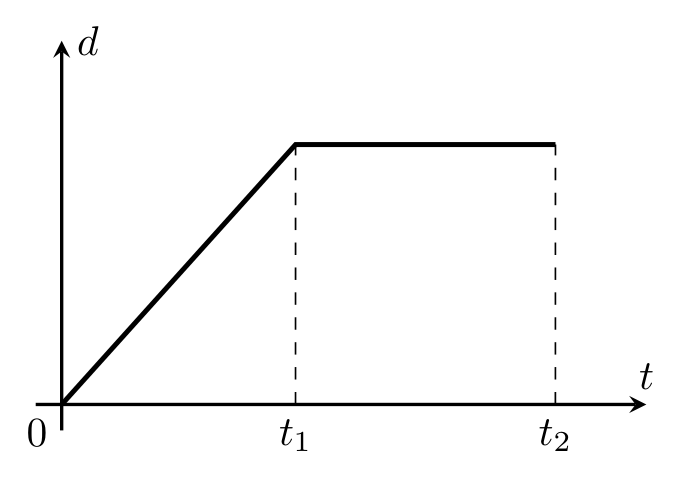
\includegraphics[width=3.8cm]{c8_dothidt.png}
		\vspace{-7pt}
	\end{center}
	\choice
	{Không có lúc nào xe chuyển động thẳng đều}
	{\True Trong khoảng thời gian từ $0$ đến $t_1$}
	{Trong khoảng thời gian từ $t_1$ đến $t_2$}
	{Trong khoảng thời gian từ $0$ đến $t_2$}
	\loigiai{}
\end{ex}

\newpage
% TRANG 2
% Câu 9
\begin{ex}
	Phát biểu nào sau đây \textbf{không đúng}?
	\choice
	{Độ dịch chuyển là vectơ nối vị trí đầu và vị trí cuối của chất điểm chuyển động}
	{Chất điểm đi trên một đường thẳng rồi quay về vị trí ban đầu thì có độ dịch chuyển bằng không}
	{\True Độ dịch chuyển bằng quãng đường đi được của chất điểm}
	{Độ dịch chuyển là đại lượng vectơ còn quãng đường đi được là đại lượng vô hướng}
	\loigiai{}
\end{ex}

% Câu 10
\begin{ex}
	Dùng thước đo có sai số dụng cụ là $1\text{ mm}$ để đo 5 lần khoảng cách giữa hai điểm M và N đều cho một giá trị như nhau là $56\text{ mm}$. Kết quả của phép đo được viết là
	\choice
	{$d = 56 \pm 0\text{ mm}$}
	{$d = 56 \pm 2\text{ mm}$}
	{\True $d = 56 \pm 1\text{ mm}$}
	{$d = 56 \pm 0{,}5\text{ mm}$}
	\loigiai{}
\end{ex}

% Câu 11
\begin{ex}
	Trong các chuyển động sau, chuyển động nào được coi là sự rơi tự do?
	\choice
	{Chiếc lá đang rơi}
	{Hạt bụi chuyển động trong không khí}
	{Vận động viên đang nhảy dù}
	{\True Quả tạ rơi trong không khí từ độ cao $50\text{ m}$}
	\loigiai{}
\end{ex}

% Câu 12
\begin{ex}
	Một ô tô đang chuyển động cùng chiều dương với tốc độ $10\text{ m/s}$ trên đoạn đường thẳng thì người lái xe hãm phanh và ô tô chuyển động chậm dần đều. Cho tới khi dừng hẳn thì ô tô đã chạy thêm được $100\text{ m}$. Gia tốc của xe có giá trị bằng
	\choice
	{$-0{,}2\text{ m/s}^2$}
	{\True $-0{,}5\text{ m/s}^2$}
	{$0{,}2\text{ m/s}^2$}
	{$0{,}5\text{ m/s}^2$}
	\loigiai{}
\end{ex}

% Câu 13
\begin{ex}
	Một vật được thả rơi tự do, tốc độ của vật khi chạm đất là $70\text{ m/s}$. Cho $g = 10\text{ m/s}^2$. Thời gian vật rơi là
	\choice
	{$3{,}5\text{ s}$}
	{\True $7\text{ s}$}
	{$8\text{ s}$}
	{$4\text{ s}$}
	\loigiai{}
\end{ex}

% Câu 14
\begin{ex}
	Chọn câu đúng. Để đo tốc độ trung bình của vật trong phòng thí nghiệm, ta cần dùng
	\choice
	{\True thước đo chiều dài và đồng hồ đo thời gian}
	{thước đo và lực kế}
	{máy bắn tốc độ}
	{lực kế và đồng hồ đo thời gian}
	\loigiai{}
\end{ex}

% Câu 15
\begin{ex}
	Cặp đồ thị nào ở hình dưới đây là của chuyển động thẳng đều?
	\begin{center}
		\vspace{-7pt}
		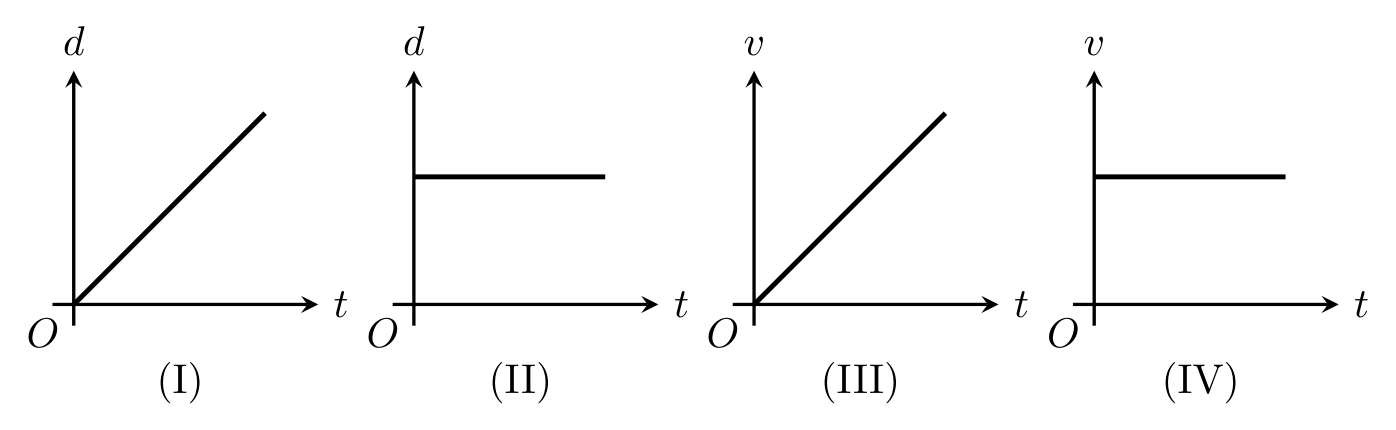
\includegraphics[width=11.5cm]{c15_dothi4.png}
		\vspace{-7pt}
	\end{center}
	\choice
	{I và III}
	{\True I và IV}
	{II và IV}
	{II và III}
	\loigiai{}
\end{ex}

% Câu 16
\begin{ex}
	Vật chuyển động thẳng nhanh dần thì vectơ gia tốc và vectơ vận tốc
	\choice
	{ngược hướng}
	{\True cùng hướng}
	{không thay đổi}
	{vuông góc}
	\loigiai{}
\end{ex}

% Câu 17
\begin{ex}
	Câu trả lời nào sau đây \textbf{Sai}. Chuyển động thẳng nhanh dần đều là chuyển động có
	\choice
	{\True quãng đường đi được của vật luôn tỉ lệ thuận với thời gian vật đi}
	{quỹ đạo là đường thẳng}
	{vectơ gia tốc của vật có độ lớn là một hằng số}
	{vận tốc có độ lớn tăng theo hàm bậc nhất đối với thời gian}
	\loigiai{}
\end{ex}

% Câu 18
\begin{ex}
	Vào lúc $10\text{ h}$, người lái xe nhìn vào tốc kế và thấy tốc kế chỉ $40\text{ km/h}$. Số liệu này cho biết
	\choice
	{tốc độ trung bình của xe}
	{vận tốc trung bình của xe}
	{\True tốc độ tức thời của xe}
	{vận tốc tức thời của xe}
	\loigiai{}
\end{ex}

\newpage
% TRANG 3
\begin{flushleft}
	{\color{blue!50!green}\fbox{\fontfamily{qag}\bfseries\selectfont PHẦN II. Câu trắc nghiệm đúng sai}}
	\textit{\small (Thí sinh trả lời từ câu 1 đến câu 4. Trong mỗi ý a), b), c), d) ở mỗi câu, thí sinh chọn đúng hoặc sai.)}
\end{flushleft}
\setcounter{ex}{0}
\setcounter{bt}{0}

% Phần II Câu 1
\begin{ex}
	Hai bạn Đức và Triết bơi trong bể bơi có chiều dài $25\text{ m}$. Hai bạn xuất phát từ đầu bể bơi đến cuối bể bơi thì Đức dừng lại nghỉ, còn Triết quay lại và tiếp tục bơi tiếp về đầu bể bơi mới nghỉ. Thời gian bơi của Đức là $25\text{ s}$; Triết bơi đi mất $23\text{ s}$ và bơi về mất $27\text{ s}$. Biết rằng Đức và Triết bơi trên một đường thẳng song song với thành bể.
	\choiceTF
	{\True Tốc độ trung bình trong thời gian $25\text{ s}$ của Đức là $1\text{ m/s}$}
	{Vận tốc trung bình trong thời gian $50\text{ s}$ của Triết là $1\text{ m/s}$}
	{Độ dịch chuyển tổng hợp của Triết có độ lớn bằng $50\text{ m}$}
	{\True Quãng đường Đức bơi được là $25\text{ m}$}
	\loigiai{}
\end{ex}

% Phần II Câu 2
\begin{ex}
	Một máy bay Boeing 747 bắt đầu xuất phát trên một đường băng thẳng dài với gia tốc $a = 2\text{ m/s}^2$. Tốc độ cần thiết để máy bay rời đường băng là $360\text{ km/h}$. Sau khi xuất phát được $30\text{ s}$ thì nhận được lệnh huỷ bay từ trạm điều khiển không lưu do thời tiết xấu nên phi công cho máy bay hãm phanh chuyển động chậm dần đều và dừng lại sau $20\text{ s}$ kể từ khi có lệnh huỷ bay.
	\choiceTF
	{\True Chuyển động của máy bay trong $30\text{ s}$ đầu tiên là chuyển động thẳng nhanh dần đều}
	{\True Tốc độ của máy bay tại thời điểm nhận được lệnh huỷ bay là $60\text{ m/s}$}
	{\True Độ lớn gia tốc của máy bay trong giai đoạn hãm phanh là $3\text{ m/s}^2$}
	{Tốc độ trung bình của máy bay trong khoảng thời gian từ lúc xuất phát cho đến khi dừng lại là $40\text{ m/s}$}
	\loigiai{}
\end{ex}

% Phần II Câu 3
\begin{ex}
	Từ các đồ thị trong hình sau. Nhận định sau đúng hay sai?
	\begin{center}
		\vspace{-7pt}
		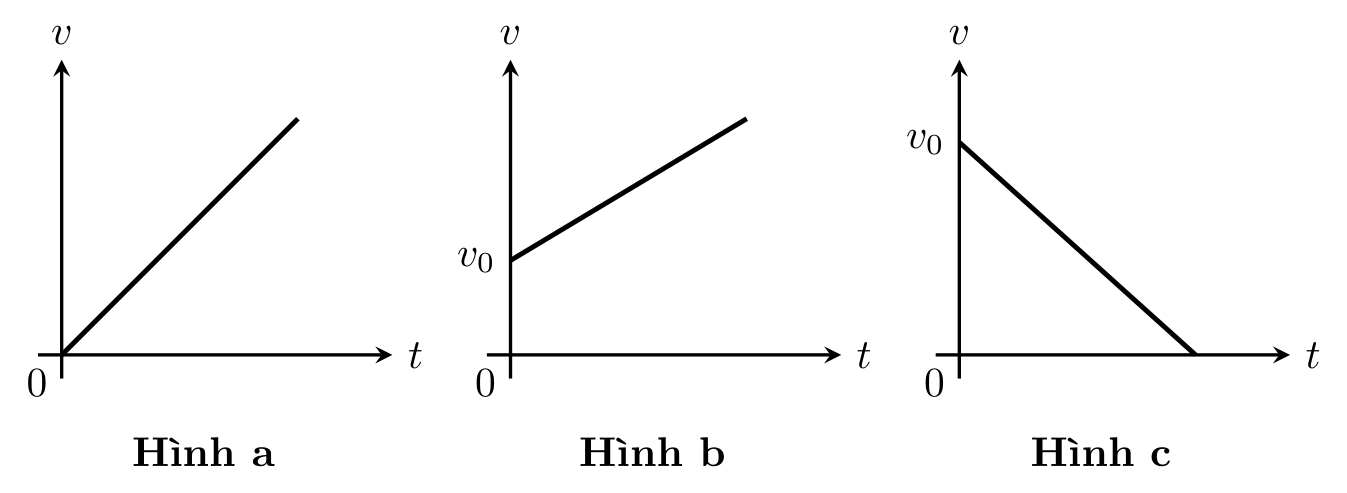
\includegraphics[width=10.5cm]{p2_c3_dothi3.png}
		\vspace{-7pt}
	\end{center}
	\choiceTF
	{\True Chuyển động thẳng nhanh dần đều là đồ thị hình a và b}
	{Đồ thị hình b có công thức vận tốc là $v = v_0 + at\ (a < 0)$}
	{\True Chuyển động thẳng chậm dần đều là đồ thị hình c}
	{Đồ thị hình c có công thức vận tốc là $v = v_0 + at\ (a > 0)$}
	\loigiai{}
\end{ex}

% Phần II Câu 4
\begin{ex}
	Bỏ qua sức cản không khí, một vật rơi tự do tại một địa điểm có độ cao $180\text{ m}$, lấy $g = 10\text{ m/s}^2$.
	\choiceTF
	{Quãng đường vật rơi được sau $3\text{ s}$ là $30\text{ m}$}
	{\True Phương rơi của vật là phương thẳng đứng}
	{\True Thời gian vật rơi hết $100\text{ m}$ cuối cùng là $2\text{ s}$}
	{Thời gian vật rơi hết quãng đường là $9\text{ s}$}
	\loigiai{}
\end{ex}

\vspace{0.1cm}
\begin{flushleft}
	{\color{blue!50!green}\fbox{\fontfamily{qag}\bfseries\selectfont PHẦN III. Câu trắc nghiệm trả lời ngắn}}
	\textit{\small (Thí sinh trả lời từ câu 1 đến câu 6.)}
\end{flushleft}
\setcounter{ex}{0}
\setcounter{bt}{0}

% Phần III Câu 1
\begin{ex}
	Cho đồ thị độ dịch chuyển theo thời gian của một vật chuyển động như hình dưới đây. Hỏi tại thời điểm $t$ bằng bao nhiêu giây thì vật đổi chiều chuyển động?
	\begin{center}
		\vspace{-7pt}
		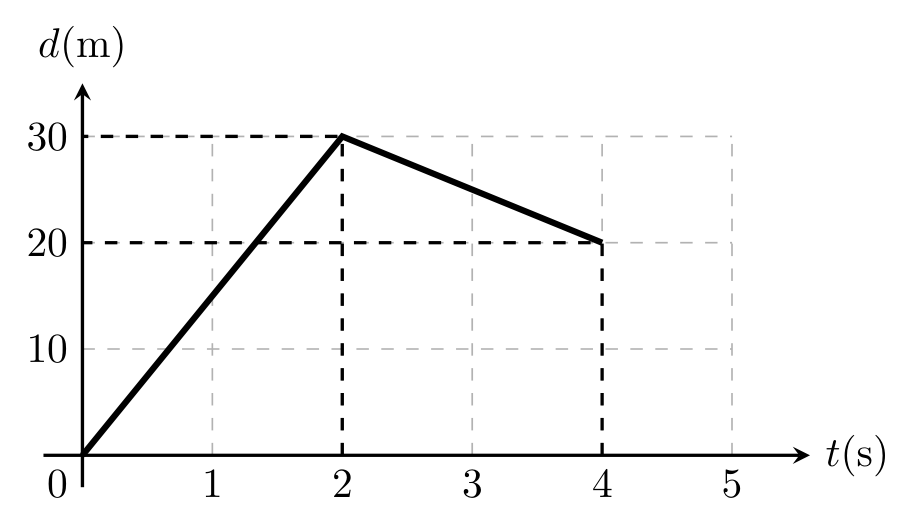
\includegraphics[width=6.2cm]{p3_c1_dothi.png}
		\vspace{-7pt}
	\end{center}
	\par\shortans[oly]{2}
	\loigiai{}
\end{ex}

\newpage
% TRANG 4
% Phần III Câu 2
\begin{ex}
	Chạy marathon là một bộ môn thể thao dưới hình thức chạy bộ được ưa chuộng nhất trên thế giới, là một môn thể thao mang đến rất nhiều lợi ích cho sức khỏe. Người tham gia có thể chạy ở các cự ly $5\text{ km}$, $10\text{ km}$ hoặc $21\text{ km}$ rồi nâng lên đường chạy dài $42\text{ km}$ trong marathon. Tùy thuộc vào thể trạng mà chúng ta lựa chọn luyện tập ở cự ly phù hợp.
	
	Pace là một từ tiếng Anh được sử dụng để chỉ nhịp điệu trong chạy bộ. Pace là số phút để một người hoàn thành $1\text{ km}$ trong khi chạy. Bạn Hương mới tập luyện nên chọn cự ly $5\text{ km}$, trong một lần tập bạn đạt được thời gian hoàn thành cự ly $5\text{ km}$ là 42 phút. Pace trung bình trong bài luyện tập chạy bộ của bạn Hương là bao nhiêu phút/km?
	\par\shortans[oly]{8,4}
	\loigiai{}
\end{ex}

% Phần III Câu 3
\begin{ex}
	Đồ thị bên dưới mô tả sự thay đổi vận tốc theo thời gian trong chuyển động của một ô tô. Gia tốc của ô tô từ $t = 15\text{ s}$ đến $t = 30\text{ s}$ có giá trị bao nhiêu $\text{m/s}^2$?
	\begin{center}
		\vspace{-7pt}
		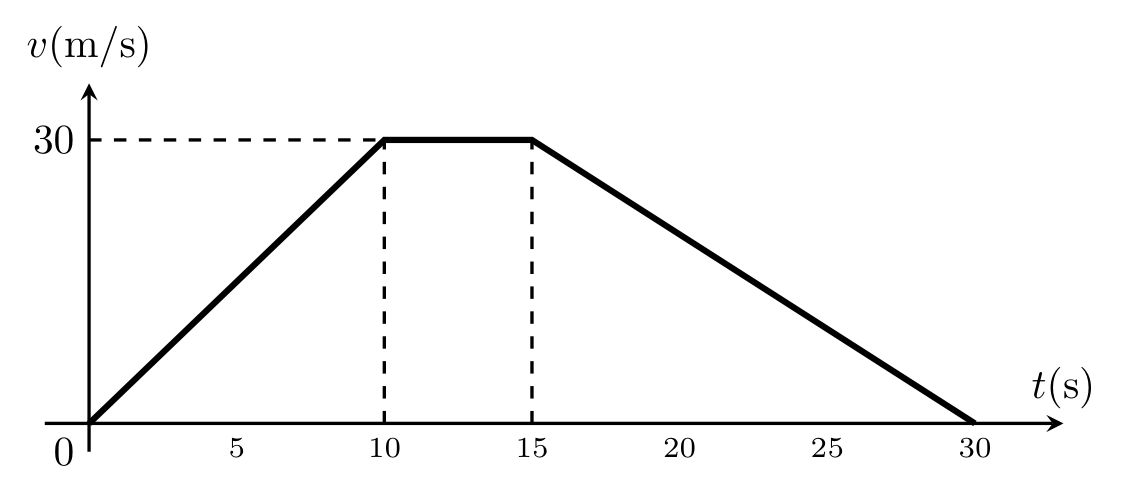
\includegraphics[width=6.6cm]{p3_c3_dothi.png}
		\vspace{-7pt}
	\end{center}
	\par\shortans[oly]{-2}
	\loigiai{}
\end{ex}

% Phần III Câu 4
\begin{ex}
	Một học sinh đo chiều dài của bàn học, kết quả thu được như sau $d = 120 \pm 1\text{ cm}$. Sai số tuyệt đối của phép đo trên là bao nhiêu cm?
	\par\shortans[oly]{1}
	\loigiai{}
\end{ex}

% Phần III Câu 5
\begin{ex}
	Đồ thị bên dưới mô tả sự thay đổi vận tốc theo thời gian trong chuyển động của một vật. Vật thay đổi tính chất chuyển động từ chuyển động thẳng đều sang chuyển động thẳng biến đổi đều ở thời điểm nào (bao nhiêu giây)?
	\begin{center}
		\vspace{-7pt}
		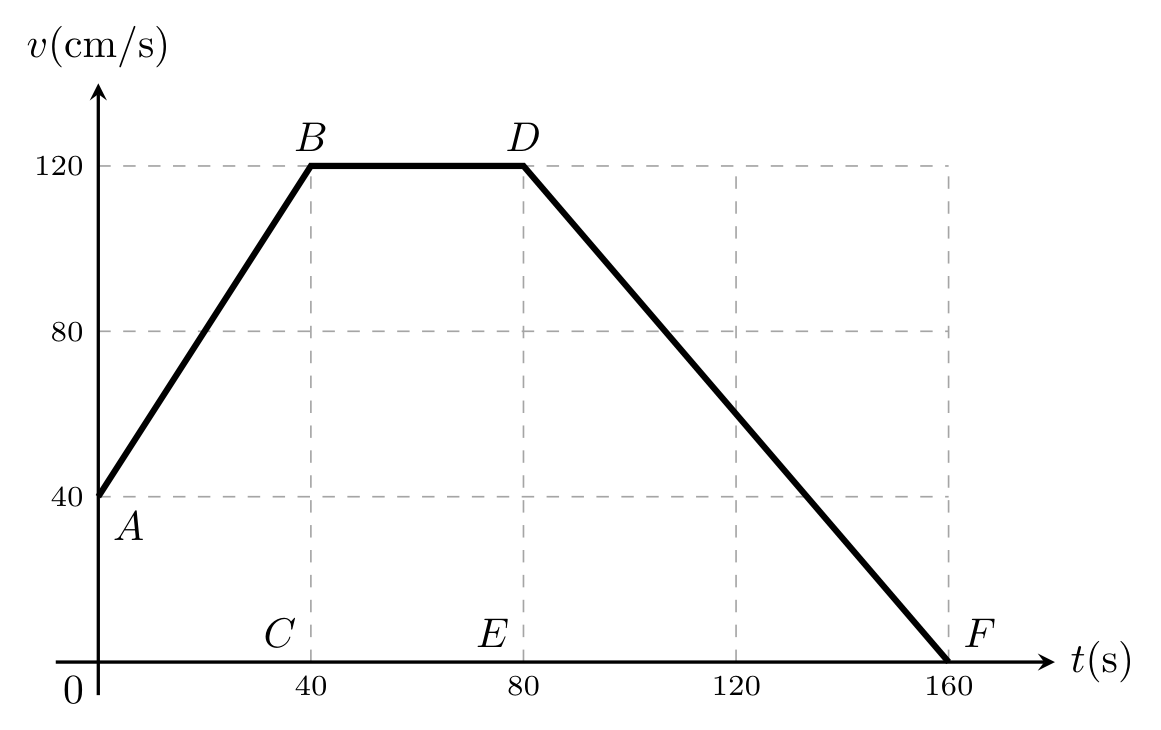
\includegraphics[width=7.2cm]{p3_c5_dothi.png}
		\vspace{-7pt}
	\end{center}
	\par\shortans[oly]{80}
	\loigiai{}
\end{ex}

% Phần III Câu 6
\begin{ex}
	Bạn Tuấn chạy bộ qua cầu đi thẳng $40\text{ m}$ theo hướng Đông, sau đó rẽ trái chạy thẳng theo hướng Bắc $100\text{ m}$ rồi quay ngược về hướng Nam $70\text{ m}$. Độ lớn độ dịch chuyển của Tuấn là bao nhiêu m?
	\par\shortans[oly]{50}
	\loigiai{}
\end{ex}

\vspace{0.3cm}
\begin{center}
	\textbf{--------- HẾT ---------}
\end{center}

\end{document}
